\subsection{Mid-infrared properties of the M31 nucleus}
\label{sect:nucleus}


Examining the spectral data cube for the nuclear region, we noticed that different spectral features
vary spatially in the near-nuclear region.
Figure \ref{nuc11} (top) shows the integrated intensity map of 11.3~$\mu$m emission made from the data cube. 
The majority of the 11.3~$\mu$m  emission is from a region 15\arcsec\ north of the nucleus and not from the nucleus itself. 
On the other hand, the centre shows little PAH emission,  but it does have silicate emission around 9.7~$\mu$m, 
which comes only from the nucleus and is not present in the North region  (see Figure \ref{nuc11}, bottom panel).%
\footnote{The spatial resolution and pixel scale of the ISOCAM data are not sufficient to resolve these two regions.}
Radial profiles of both the nuclear and north sources have full widths at half maximum (FWHM) of 5--7\arcsec\ 
depending on the wavelength, while the SL PSF FWHM is 2.5--3\arcsec; therefore both sources are
marginally spatially resolved.  
We extracted spectra from the centre and the North regions using  $9\arcsec \times 9\arcsec$ 
square apertures as shown in Figure \ref{nuc11}. 

% SPW had some comments on number of ticks in these -- prob going to ignore
\begin{figure}
\centering
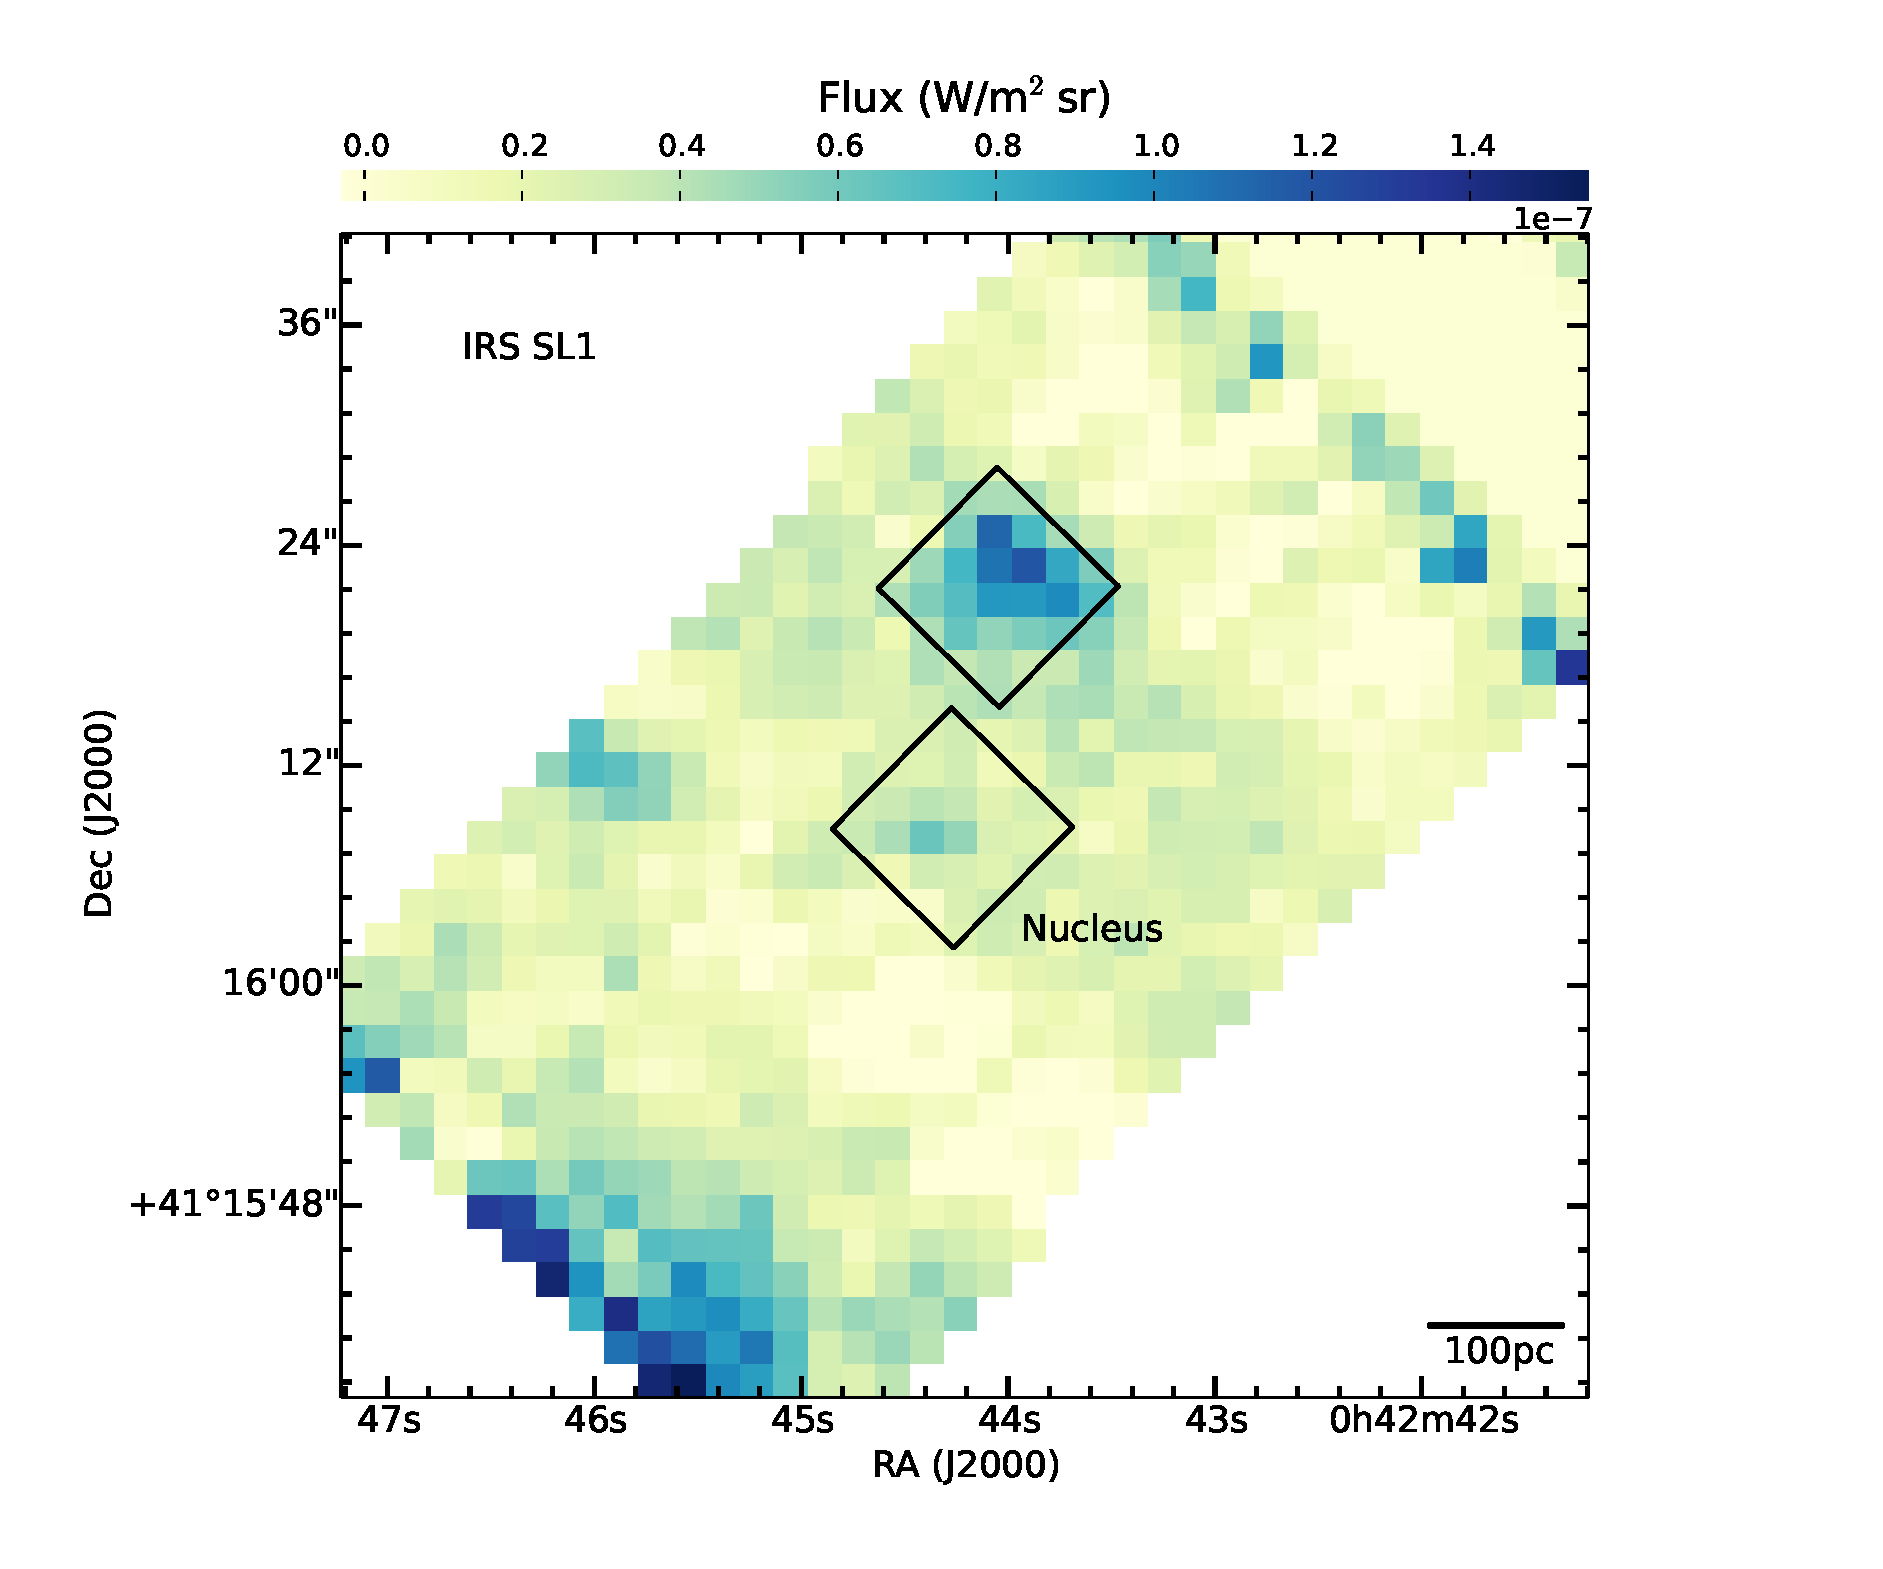
\includegraphics[width = 8 cm]{./nuc11_3.eps}
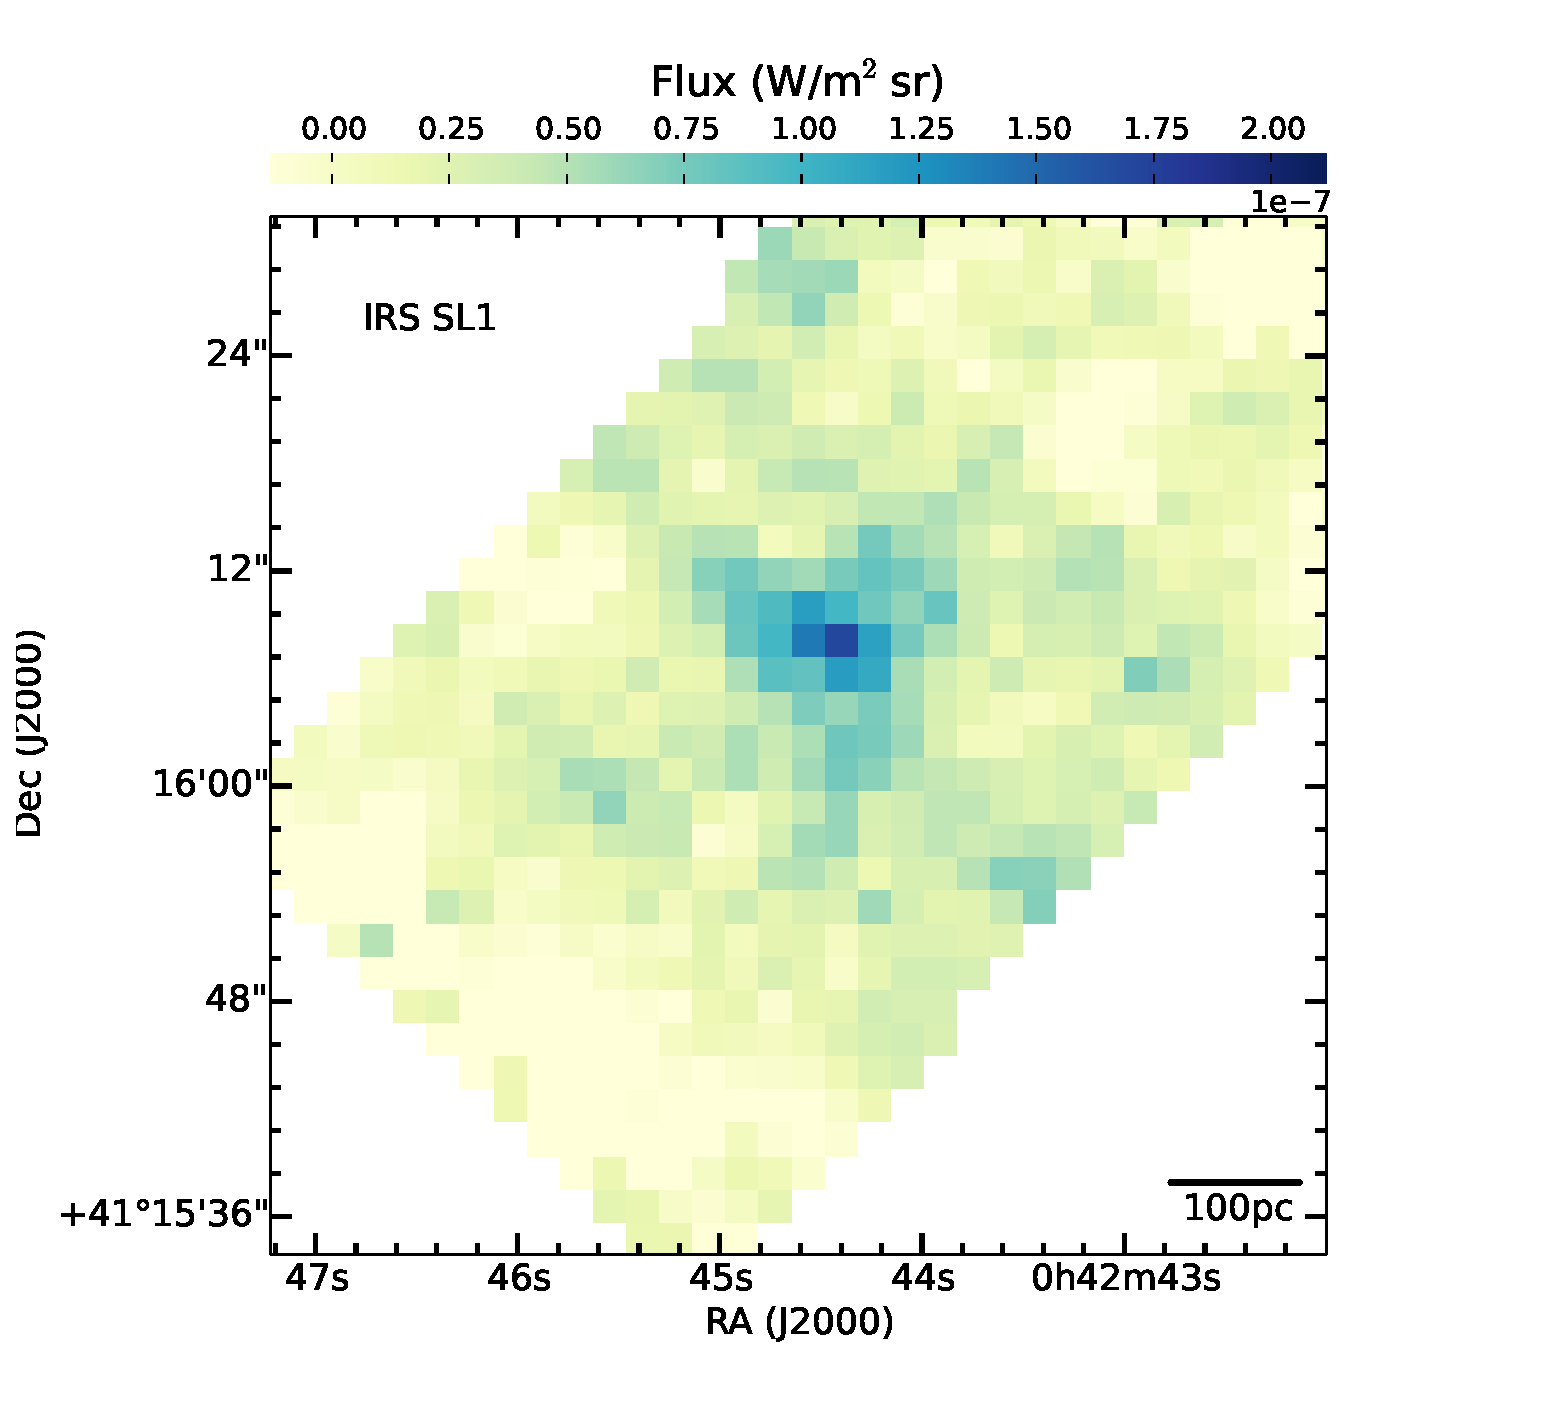
\includegraphics[scale = 0.3]{./NUCsilicate.eps}
\caption{(Top): Intensity variation of 11.3~$\mu$m emission around the nucleus of M31. 
Two black boxes are the apertures (centre and north region) used to extract spectra in Figure \ref{smithspec}. 
The centre of the nucleus is at R.A. $00^{\rm h}42^{\rm m}44\fs35$, Dec. $+41\degr16\arcmin08\farcs5$ \citep{NucleusREF}. % TODO: mark in figure. Is this the stellar centre?
(Bottom:) Integrated strength of the silicate emission (from 9 to 11~$\mu$m, continuum subtracted) near the M31 nucleus.} % CHECK - is this continuum subtracted?
\label{nuc11}
\end{figure}

Figure~\ref{fig:nuc_detail} shows the spectra extracted from the two regions near the nucleus.
Like the ISOCAM spectrum (Figure~\ref{ISOnIRS}), the  {\em Spitzer} spectra show a blue
continuum, PAH features weak or absent at 6--8~$\mu$m  but detectable at 11.3~$\mu$m, and detectable atomic fine structure lines.
{\bf here is where Els makes it all clear.}

\begin{figure}
\centering
\includegraphics[width = 8 cm]{./fig_sp_m31_nucleus.eps}
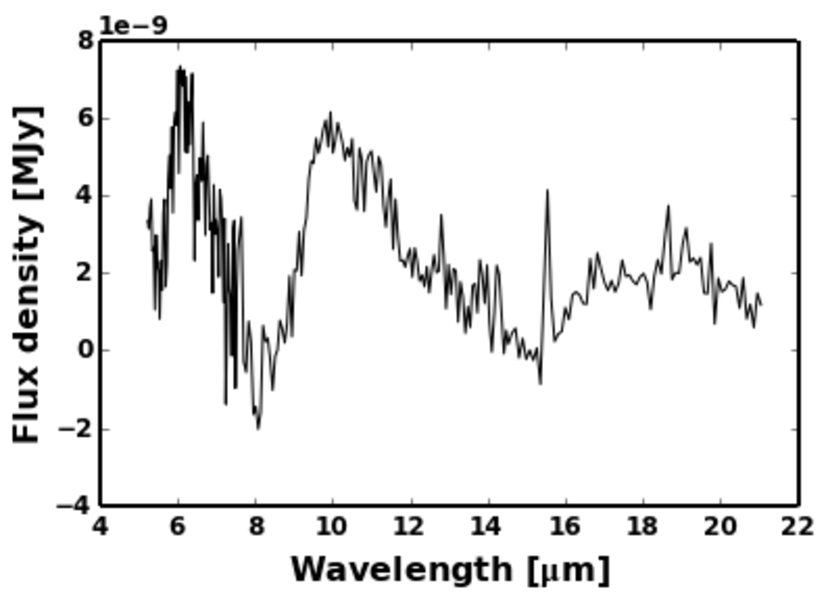
\includegraphics[width = 8 cm]{./nuc_ctr_contsub.pdf}
\caption{Top: PAHFit result for centre and north spectra (placeholder, to be improved).
Bottom: continuum-subtracted centre spectrum.}
\label{fig:nuc_detail}
\end{figure}


\begin{figure*}
\centering
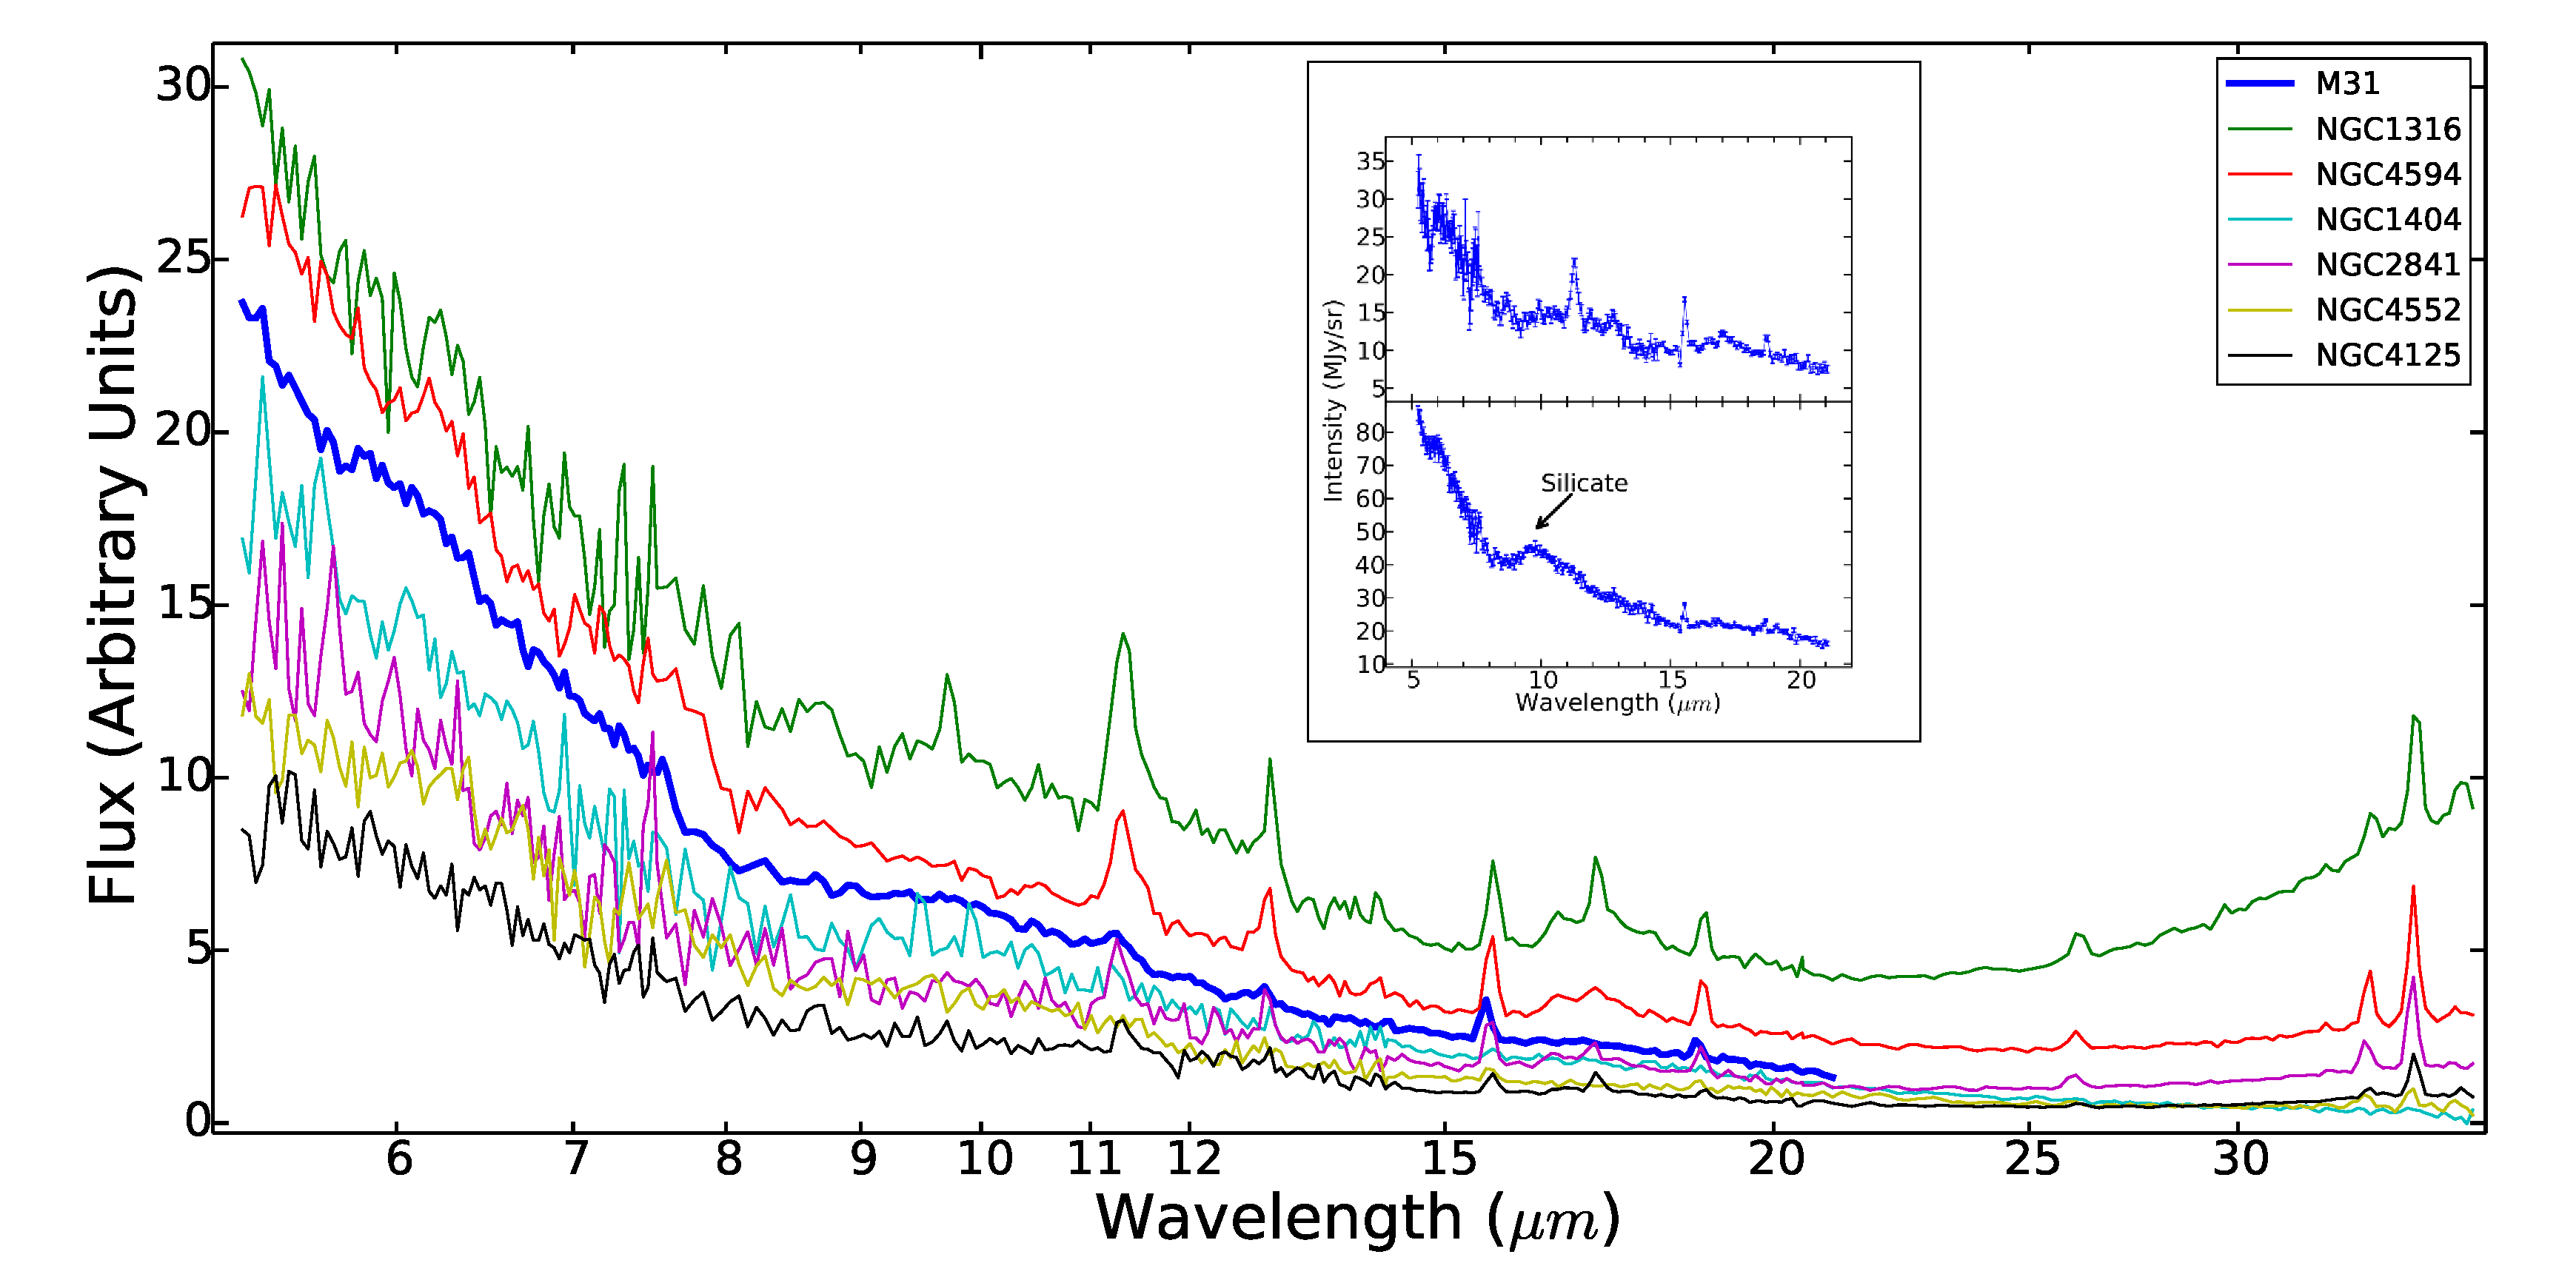
\includegraphics[height = 8 cm]{./SINGSspec.eps}
\caption{Mid-infrared spectrum of the nucleus of M31 (blue) over-plotted with spectra extracted close to the nuclei of 6 nearby galaxies which have 
AGN activity \citep{Smith:2007lr}. NGC 4552, NGC 1404 and NGC 4125 are elliptical galaxies and NGC 4594 and NGC 2841 are spiral galaxies. 
NGC 1316 is a lenticular galaxy. The inset shows the spectra extracted from the centre region of the M31 nucleus (bottom) and from the north region (top) 
shown in Figure \ref{nuc11}.}
\label{smithspec}
\end{figure*}

Figure \ref{smithspec} compares the full 30\arcsec $\times$ 50\arcsec\ M31 nuclear spectrum with
the North and central region spectra (inset, top and bottom). Also shown are nuclear spectra
from six SINGS galaxies with similar spectral shapes \citep{Smith:2007lr}.% 
\footnote{The IRS spectra for the SINGS galaxies were extracted over areas ranging from 2 to 8 kpc$^2$, whereas the M31
nucleus spectrum covers a much smaller area (0.02~kpc$^2$).}
The strong 11.3~$\mu$m peak  and weak 6--8~$\mu$m features are  seen  in the
North spectrum, while a silicate emission feature is evident in the central spectrum.
The SINGS galaxies share similar PAH feature characteristics to the M31 spectrum, although none
contains obvious silicate emission. The nuclear spectrum of M81 presented by \citet{Smith2010}
shows both 11.3~$\mu$m  and silicate emission; in common with some of the SINGS galaxies,
it also has strong atomic lines (e.g. [Ne {\sc ii}]~12.8~$\mu$m) not present in the M31 spectrum.


All of the comparison galaxies discussed above have some type of low-luminosity active galactic nucleus (LLAGN).
The SINGS galaxies with similar spectral shapes include  three elliptical galaxies, two spirals, and a lenticular;
there is some disagreement  \citep{kennicutt03,Smith:2007lr, moustakas2010} are in some disagreement over the
exact nuclear spectral types of these six galaxies.  All are classified as some form of LLAGN
such as Seyfert or LINER \citep[luminous AGNs were intentionally omitted from the SINGS sample;][]{kennicutt03}, although they are
by no means the only LLAGNs in the SINGS sample.
Published estimates of the black hole masses for these galaxies range from $1.5-5.5\times10^{8}$~M$_{\sun}$
\citep[for NGC~1316 and NGC~4595, respectively]{nowak08, kormendy88}, or about $1-4\times$ that of M31.
M81 is classified as a LINER, with a black hole mass of $7\times10^7$~M$_{\sun}$ \citep{devereux03}.
\citet{Li09} concluded that the central black hole in M31 (M31*) is currently inactive, with direct observational signatures seen only
at radio and X--ray wavelengths, so finding additional signatures in the mid-infrared is of great interest.
To our knowledge, no such signatures have been reported; broadband mid-infrared imaging of the central 
regions of M31 \citep{davidge06,Barmby2006lr} did not identify unambiguous nuclear emission. The bluest
part of the spectrum in Figure~\ref{fig:nuc_detail} is dominated by the  continuum, in agreement with the
expectation that stellar light dominates the nucleus at these wavelengths.


Could radiation from M31* be responsible for the suppression of the  6--8~$\mu$m PAH features compared
to the 11.3~$\mu$m feature?
As discussed by  \citet{Smith:2007lr} and \citet{Smith2010}, inferring such a suppression must be done with caution, 
because the 6--8~$\mu$m features are more susceptible to dilution by the stellar continuum. 
Several connections between PAH suppression and the presence of an AGN are possible, including destruction of small 
or charged PAH molecules by a hard radiation field, or weak ultraviolet continuum from low star formation rates 
leading to reduce PAH excitation \citep{Smith:2007lr}.  In the latter case, the AGN is not the cause of
the suppressed  6--8~$\mu$m features but rather is only detectable when the nuclear star formation rate is low.
Previous work has found low rates of star formation in the centre of M31: although \citet{Melchior2013} found a significant 
amount of cold gas in the centre of the galaxy, this gas does not appear to be associated with current star formation \citep[see also][]{Li09}.
In modelling the far-infrared spectral energy distribution, \cite{Groves2012} found that  
the old stellar population in the M31 bulge is sufficient  to heat the observed dust; no young stellar population is needed.
We conclude that PAH feature ratios cannot provide direct evidence for radiation from M31*.


Detection of silicate emission in the M31 nuclear spectrum is another possible indicator of nuclear accretion.
Silicate emission is not very common in integrated spectra of galaxies \citep{Spoon2007} but is seen in luminous 
quasar spectra \citep{Hill14} and, as mentioned above, in the spectrum of the M81 nucleus. 
In the unified model of AGNs, an obscuring torus viewed face-on would be expected to show silicate emission
\citep{AGNtypes1995, AGNref}; however such a view would also be expected to show forbidden atomic lines such as [Ne~{\sc v}] and [S~{\sc iv}],
not seen in the M31 spectrum. Alternatively, \citet{Mason2012} explained that low-luminosity AGNs cannot 
host a Seyfert-like obscuring torus because of their optically thin dust and low dust-to-gas ratio, but can show
silicate emission that originates in the optically thin hot dust around the torus.  The first detection of such silicate emission was 
reported by \citet{Sturm2005} from the low-ionization nuclear emission-line region (LINER) galaxy NGC~3998, and 
\citealt{Mason2012}  observed that  9.7~$\mu$m silicate emission is present in many LLAGNs. 
To quantify the magnitude of the silicate emission in mid-infrared spectra, \citet{Smith2010} defined
the linear slope parameter $\gamma810 =[F_{\nu}(10\mu{\rm m}) -F_{\nu}(8\mu{\rm m})]/2F_{\nu}(9\mu{\rm m})$,
with positive values signifying silicate emission and negative values absorption. They found the M81 nucleus to have
$\gamma810=0.37\pm0.04$. For the M31 centre (9\arcsec $\times$ 9\arcsec) spectrum, we computed  $\gamma810 =0.01\pm 0.03$,
indicative of neither absorption nor emission. However, for the continuum-subtracted spectrum, we measured   $\gamma810 =1.6\pm 0.4$,
a much stronger indication that silicate emission is detected from M31*.

Measuring the radiated power from the M31 central engine can constrain the geometry and history of the emitting region. 
As discussed by \citet{spinoglio95}, for both active and normal galaxies, the 12~$\mu$m luminosity 
is about 7\% of the bolometric luminosity. With the important caveat that we are discussing only the nucleus,
and not the entire galaxy, we  can use the infrared spectrum to estimate the bolometric luminosity  of the M31 nucleus.
For the centre spectrum, we measure a 12~$\mu$m flux density of 
$0.062 \pm 0.002$~Jy, which corresponds to a 12~$\mu$m luminosity of $(1.13\pm0.03) \times10^{39}$ erg~s$^{-1}$ and a bolometric luminosity
of  $(1.62\pm0.01) \times10^{40}$ erg~s$^{-1}$ ($\log L_{\rm bol} = 40.21$). 
This value is well within the range defined for low-luminosity AGN \citep[$\log L_{\rm bol} <42$][]{Mason2012}, and
implies an Eddington ratio $L_{\rm bol}/L_{\rm Edd} \sim 10^{-7}$ for a black hole mass of $10^8$~M$_{\sun}$. 
Although the bolometric luminosity estimated from the mid-infrared is a factor of $10^3$ times the bolometric
luminosity estimated from the X--ray flux by \citet{Li09}, it certainly agrees with the general conclusion that the M31 nucleus radiates extremely inefficiently.
A high infrared-to-X--ray ratio could indicate that the nucleus was brighter in the recent past and is now cooling;
detailed modeling of the nucleus would require better constraints on the spectral energy distribution and is hence beyond the scope of this work.

